
\chapter{Diseño e implementación} % Main chapter title
En este capítulo se abordará la descripción de la arquitectura general del sistema, arquitectura del firmware, código de los controladores desarrollados, desarrollo del hardware y la configuración de la plataforma IoT.
\label{Chapter3} % Change X to a consecutive number; for referencing this chapter elsewhere, use \ref{ChapterX}

\definecolor{mygreen}{rgb}{0,0.6,0}
\definecolor{mygray}{rgb}{0.5,0.5,0.5}
\definecolor{mymauve}{rgb}{0.58,0,0.82}

%%%%%%%%%%%%%%%%%%%%%%%%%%%%%%%%%%%%%%%%%%%%%%%%%%%%%%%%%%%%%%%%%%%%%%%%%%%%%
% parámetros para configurar el formato del código en los entornos lstlisting
%%%%%%%%%%%%%%%%%%%%%%%%%%%%%%%%%%%%%%%%%%%%%%%%%%%%%%%%%%%%%%%%%%%%%%%%%%%%%
\lstset{ %
  backgroundcolor=\color{white},   % choose the background color; you must add \usepackage{color} or \usepackage{xcolor}
  basicstyle=\footnotesize,        % the size of the fonts that are used for the code
  breakatwhitespace=false,         % sets if automatic breaks should only happen at whitespace
  breaklines=true,                 % sets automatic line breaking
  captionpos=b,                    % sets the caption-position to bottom
  commentstyle=\color{mygreen},    % comment style
  deletekeywords={...},            % if you want to delete keywords from the given language
  %escapeinside={\%*}{*)},          % if you want to add LaTeX within your code
  %extendedchars=true,              % lets you use non-ASCII characters; for 8-bits encodings only, does not work with UTF-8
  %frame=single,	                % adds a frame around the code
  keepspaces=true,                 % keeps spaces in text, useful for keeping indentation of code (possibly needs columns=flexible)
  keywordstyle=\color{blue},       % keyword style
  language=[ANSI]C,                % the language of the code
  %otherkeywords={*,...},           % if you want to add more keywords to the set
  numbers=left,                    % where to put the line-numbers; possible values are (none, left, right)
  numbersep=5pt,                   % how far the line-numbers are from the code
  numberstyle=\tiny\color{mygray}, % the style that is used for the line-numbers
  rulecolor=\color{black},         % if not set, the frame-color may be changed on line-breaks within not-black text (e.g. comments (green here))
  showspaces=false,                % show spaces everywhere adding particular underscores; it overrides 'showstringspaces'
  showstringspaces=false,          % underline spaces within strings only
  showtabs=false,                  % show tabs within strings adding particular underscores
  stepnumber=1,                    % the step between two line-numbers. If it's 1, each line will be numbered
  stringstyle=\color{mymauve},     % string literal style
  tabsize=2,	                   % sets default tabsize to 2 spaces
  title=\lstname,                  % show the filename of files included with \lstinputlisting; also try caption instead of title
  morecomment=[s]{/*}{*/}
}


%----------------------------------------------------------------------------------------
%	SECTION 1
%----------------------------------------------------------------------------------------
\section{Diagrama de bloques general del sistema}

En la figura \ref{fig:Diagrama general del sistema IoT} se muestra el diagrama en bloques general del sistema donde se describe la arquitectura IoT aplicada al proyecto que consta de tres capas: percepción, red y aplicación.

\begin{figure}[h]
	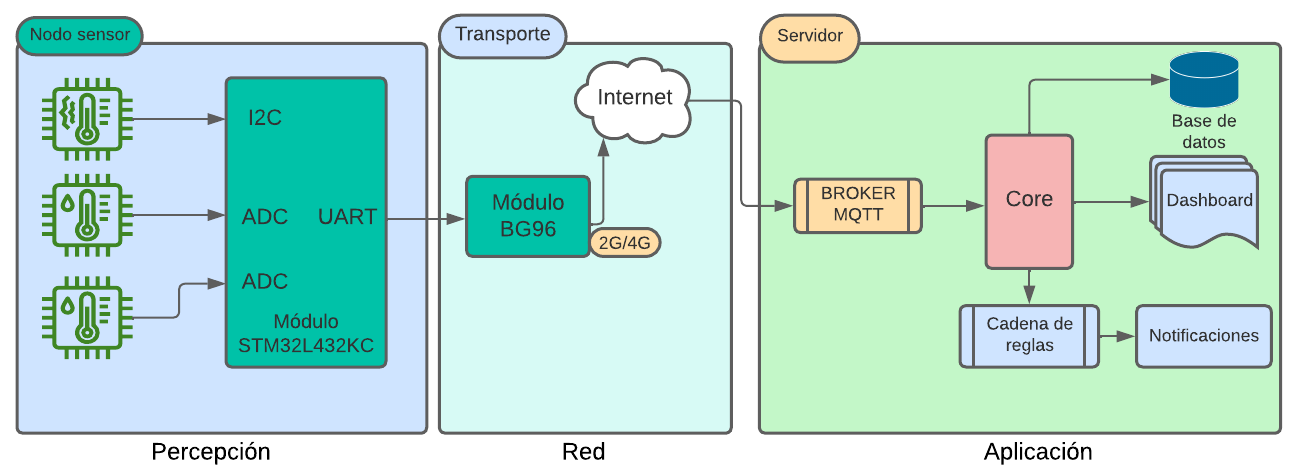
\includegraphics[width=\textwidth, height=8cm]{./Figures/DiagramaDelSistema.png}
	\caption{Diagrama general del sistema IoT.}
	\label{fig:Diagrama general del sistema IoT}
\end{figure}

En cada una de las capas se despliegan tecnologías y componentes de hardware y software. A continuación se describe cada una de las capas.

\begin{itemize}
	\item \textbf{Capa de percepción}: En la capa de percepción se encuentra el nodo sensor que es el encargado de medir las variables físicas, hacer un preprocesamiento y posteriormente enviar los datos a la capa de red. Para su desarrollo se utilizó la tarjeta de prueba STM32L432KC que contiene el firmware del sistema, se utilizaron los siguientes sensores: sensor de humedad y temperatura ambiente AHT10, sensor de humedad de suelo HL-69 y el sensor de luz UV ML8511.
  \item \textbf{Capa de red}: En cuanto a la red se utilizó un módulo quectel BG96 que puede conectarse a la red 2G, 4G, NB-IoT automáticamente dependiendo del nivel de la red en el lugar de la implementación del nodo sensor, se comunica con el microcontrolador por comandos AT por puerto UART.
  \item \textbf{Capa de aplicación}: En la capa de aplicación, se utilizó ThingsBoard como plataforma IoT que nos brinda los microservicios de broker MQTT como puerta de entrada al servidor, base de datos para el almacenamiento, nos brinda la interfaz gráfica para la visualización de los datos y nos permite gestionar las alarmas del sistema.

\end{itemize}

\section{Arquitectura de firmware}
El desarrollo del firmware fue la tarea más compleja del proyecto debido a que uno de los objetivos fue lograr un firmware estructurado en capas para facilitar el desarrollo y reducir la complejidad del código como se muestra en la figura \ref{fig:Capas del firmware}.

\begin{figure}[h]
  \centering
	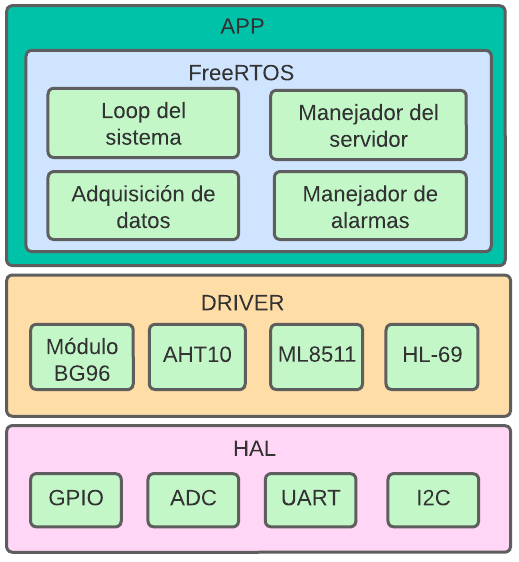
\includegraphics[width=7cm, height=8cm]{./Figures/Capas del firmware.png}
	\caption{Capas del firmware.}
	\label{fig:Capas del firmware}
\end{figure}

\subsection{Capa HAL} 
La capa HAL(\textit{Hardware Abstraction Layer}) proporcionada por el fabricante del microcontrolador  es la más baja del sistema, proporciona a las capas superiores la capacidad de interactuar con los periféricos del  microcontrolador a través de funciones en lenguaje C.
\begin{itemize}
  \item GPIO: La API proporciona funciones  para gestionar las entradas y salidas del microcontrolador. Fueron utilizadas por la capa de APP para el control de los leds de debug y para el encendido y reset del módulo de comunicación.
  \item ADC: Proporcionan funciones para la configuración, lectura y escritura de los pines de microcontroladora para trabajar con señales analógicas. Se utilizaron estas funciones para hacer la lectura de los sensores de humedad del suelo y el sensor de luz UV.
  \item UART: Brinda funciones para la lectura y escritura del puerto UART del microcontrolador. El firmware utiliza estas funciones para la comunicación con el módulo BG96.
  \item I2C: sProporciona funciones para la lectura y escritura por protocolo I2C. El driver del sensor de AHT10 utiliza estas funciones para hacer la lectura de los datos.
    
\end{itemize}

\subsection{Capa drivers} 
La capa drivers(\textit{manejador de dispositivos}) está compuesta por los manejadores que se desarrollaron para interactuar con el hardware externo al microcontrolador. Se desarrollaron drivers para el modulo de comunicacion BG96, AHT10.
\begin{itemize}
  \item Driver BG96: Las funciones más importantes que proporciona el driver:
  \begin{itemize}
    \item Estado del módulo.
    \item Descripcion del modulo.
    \item Configuración APN de la red.
    \item Conexión TCP.
    \item Conexión al broker MQTT.
  \end{itemize}
  \item Driver AHT10: Se desarrollo utilizando la hoja de datos del sensor, proporciona las funciones mas importante de inicializacion y lectura de humedad y temperatura obtenidos por el sensor.
  \item ML8511: Se escribio una funcion que permite convertir los datos obtenidos de forma analogica a valores significativos de radiacion UV.
  \item HL-69: Se escribio una funcion que permite convertir los datos obtenidos de forma analogica a valores significativos humedad del suelo. 
\end{itemize}

\subsection{Capa aplicación} 
La capa de APP o aplicación  es la de mayor nivel jerárquico. Se desarrolló sobre freeRTOS 
que nos permite hacer un código más escalable.
Se implementaron cuatro tareas.
\begin{itemize}
    \item Loop del sistema: Esta tarea es la que nos da la secuencialidad del sistema.
    \item Manejador del  servidor: Se encarga de manejar la conexión a la red y al broker MQTT.
    \item Adquisición de datos: Se encarga de hacer la lectura de los sensores.
    \item Manejador de alarmas: Esta tarea se encarga de hacer el control de las alarmas del sistema.
\end{itemize}
\clearpage

\section{Desarrollo del firmware}

Para el desarrollo del firmware se utilizo STM32CubeIDE que es el entorno de desarrollo oficial de STMicroelectronic.

El firmware fue desarrollado sobre freeRTOS, se utilizaron algunas de sus funcionanlidades como colas, semaforos, tareas, interrupciones.

En la figura \ref{fig:Df inicio firmware}  se muestra en diagrama de flujo de inicion del firmware.

\begin{figure}[htbp]
  \centering
	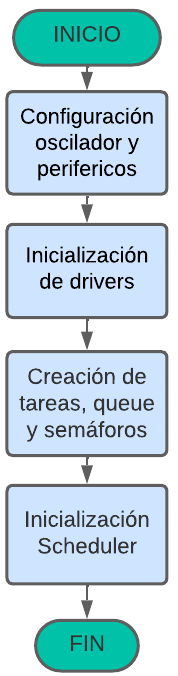
\includegraphics[width=3cm]{./Figures/DF inicio firmware.png}
	\caption{Diagrama de flujo inicio firmware.}
	\label{fig:Df inicio firmware}
\end{figure}

Lo primero que el firmware realiza es la configuración del hardware del microcontrolador, luego se inicializan los drivers del modulo de comunicacion celular BG96 y el driver del sensor de humedad y temperatura AHT10, posteriormente se crean las tareas, colas y los semáforos del sistema y finalmente se da el control del sistema al scheduler del sistema operativo. 

Para el control del sistema se crearon cuatro tareas sobre freeRTOS, que se comunican y sincronizan a través de colas y semáforos.

\subsection{Tarea loop del sistema} 

La secuencialidad del sistema es manejada por la tarea loop, la figura \ref{fig:Df tarea loop sistema} muestra el diagrama de flujo de la tarea loop.
La tarea comienza iniciando el timer del sistema el cual es el encargado de manejar el tiempo en que se repetira el ciclo de la tarea loop, luego la tarea se bloquea en el un semáforo que sera desbloqueada en el momento de la ejecución del handler de la interrupción del timer, luego se envia datos por la cola de adquisición de datos y server mqtt para levantar el servidor y la tarea se vuelve a bloquear en el semáforo, cuando se desbloquea pregunta si se logró levantar el servidor si se logró se manda un mensaje por la cola de server mqtt con el evento de enviar datos y se bloquea nuevamente pero si no se logró levantar el servidor no se enviaran datos, luego se envía un evento a la cola de alarmas y  se bloquea nuevamente esperando que envíen las alarmas, cuando se desbloquea se manda un evento a la cola de server mqtt para desconectar el servidor y se bloquea la tarea en el semáforo esperando la desconexión  finalmente se inicia nuevamente el timer y mandamos al sistema a modo de bajo consumo.

\begin{figure}[h]  
\centering
	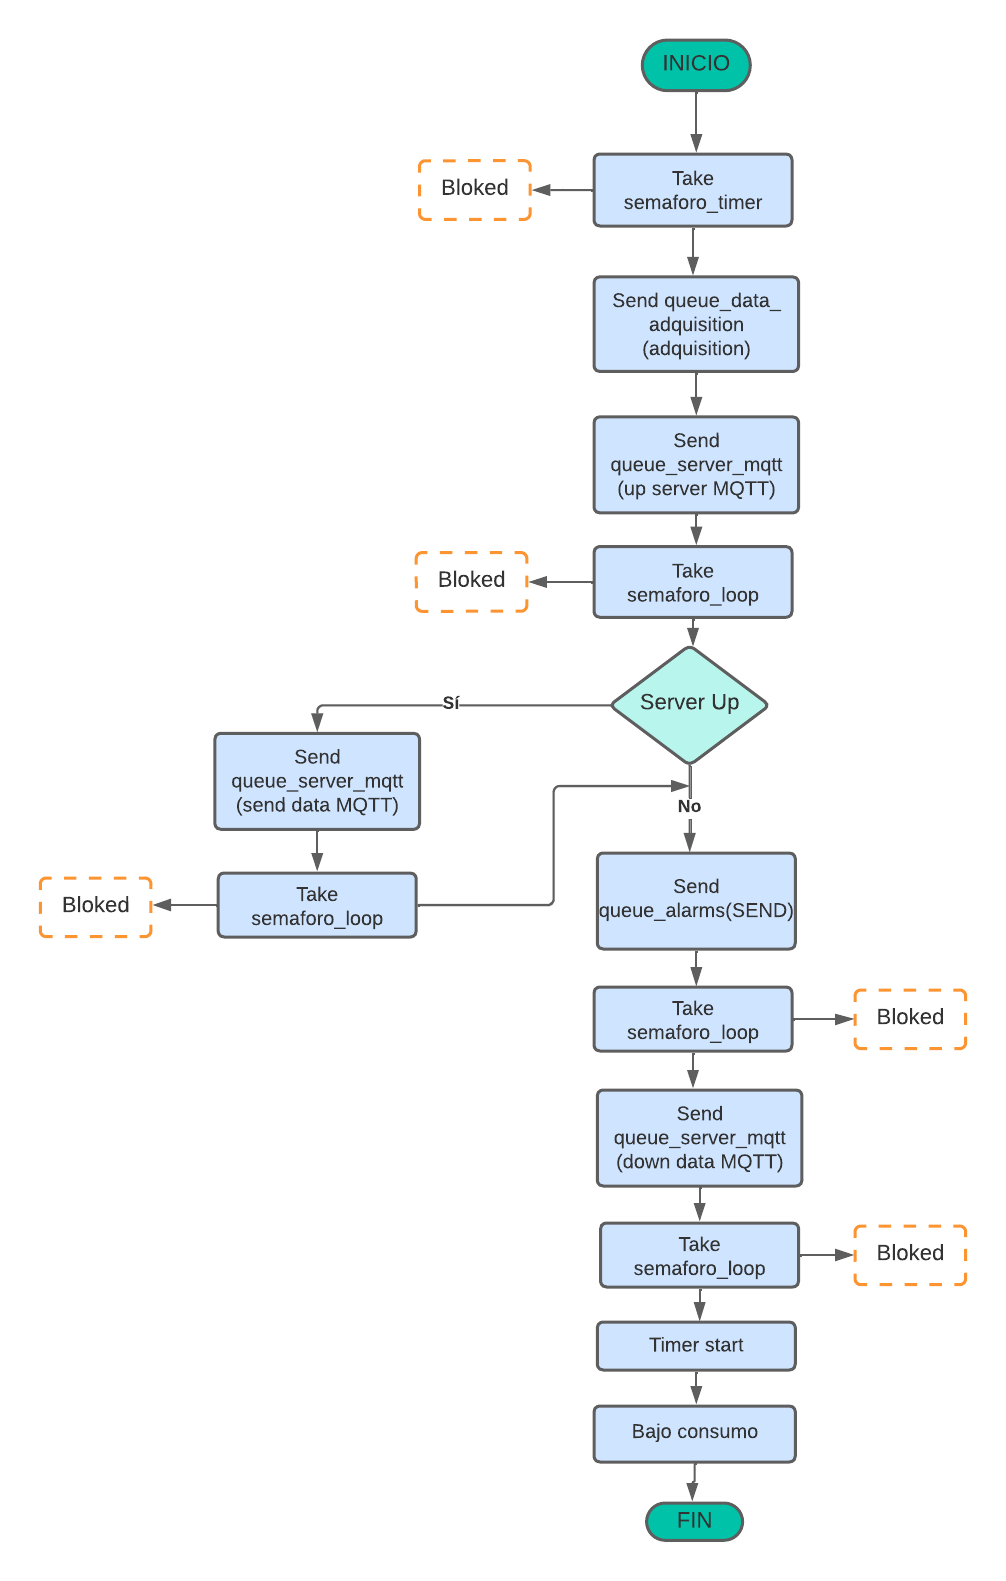
\includegraphics[width=12cm, height=16cm]{./Figures/DF task loop.png}
	\caption{Diagrama de flujo tarea loop.}
	\label{fig:Df tarea loop sistema}
\end{figure}

\subsection{Tarea adquisicion de datos} 
La figura \ref{fig:Df tarea adquisicion} muestra la secuencia repetitiva que realiza la tarea de adquisición de datos, la tarea inicia creando algunas variables locales que se utilizara en la tarea,luego revisa si hay algún dato en la cola de adquisición de datos si no hay datos la tarea se bloquea pero si existen datos en la cola se realiza la lectura de todos los sensores para posteriormente enviar los datos recolectados por la cola de data y alarmas.

\begin{figure}[h]
  \centering
	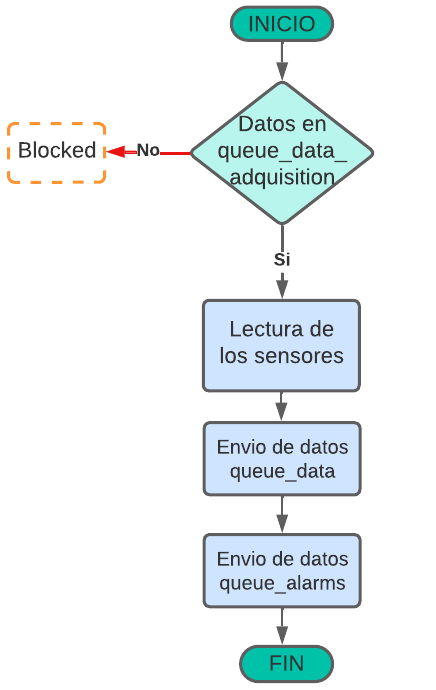
\includegraphics[width=5cm, height=7cm]{./Figures/DF task adquisicion.png}
	\caption{Diagrama de flujo tarea de adquisicion de datos.}
	\label{fig:Df tarea adquisicion}
\end{figure}

\subsection{Tarea manejador de alarmas} 
El control de las alarmas se realiza a través de la tarea de manejador de alarmas la figura \ref{fig:Df tarea alarmas} describe la secuencia de la tarea, al entrar al bucle infinito lo primero que se realiza es revisar si existe algún dato en la cola de alarmas si no hay datos la tarea se bloquea hasta que alguien envíe un dato a la cola, si hay datos se pregunta qué evento contiene el dato recibido, si el evento es de MONITOREAR lo que se hace es ver si el dato del sensor de humedad es menor al valor minimo aceptado si es así se pone  una variable en alto advirtiendo al sistema que hay una alarma, si se recibió el evento de SEND se revisa si hay alarmas activas si hay se envía un mensaje de alarma por mensaje de texto al número configurado al inicio del sistema.
\begin{figure}[h]
  \centering
	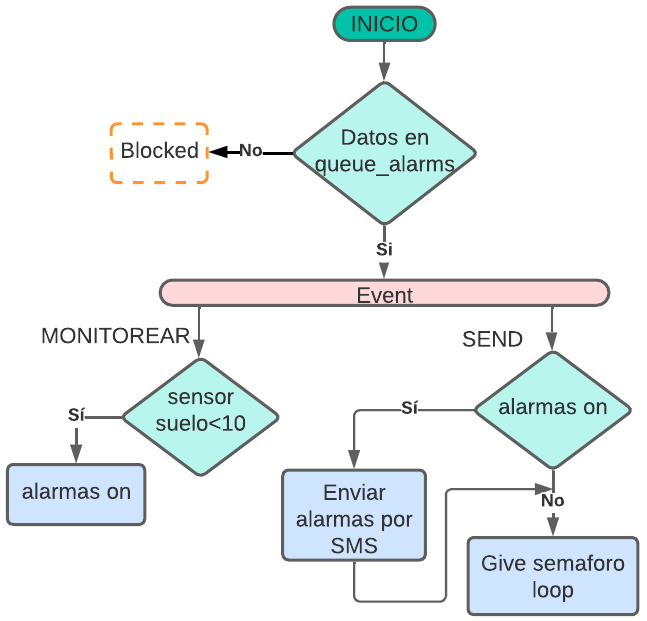
\includegraphics[width=6cm, height=6cm]{./Figures/DF_alarms.png}
	\caption{Diagrama de flujo tarea manejador de alarmas.}
	\label{fig:Df tarea alarmas}
\end{figure}

\subsection{Tarea manejador del servidor } 
La última tarea que se implementó es la tarea que maneja la conexión del servidor que se describe en la figura \ref{fig:Df tarea conexion}.
La tarea comienza esperando datos en la cola de servidor mqtt si no hay datos la tarea se bloquea, si hay datos se revisa que evento es el que se recibió tenemos tres posibles eventos UP, DOWN y SEND, si recibimos el evento de UP la tarea entra a una máquina de estados para levantar el servidor la figura \ref{fig:Maquina de estados up servidor} muestra la máquina de estados del evento UP, si el evento es de DOWN la tarea ejecuta la máquina de estados que se ve en la figura \ref{fig:Maquina de estados dowm servidor} y el evento es SEND la tarea espera que existan datos en la cola de data para así armar la trama y publicar los datos al broker MQTT.

\begin{figure}[h]
  \centering
	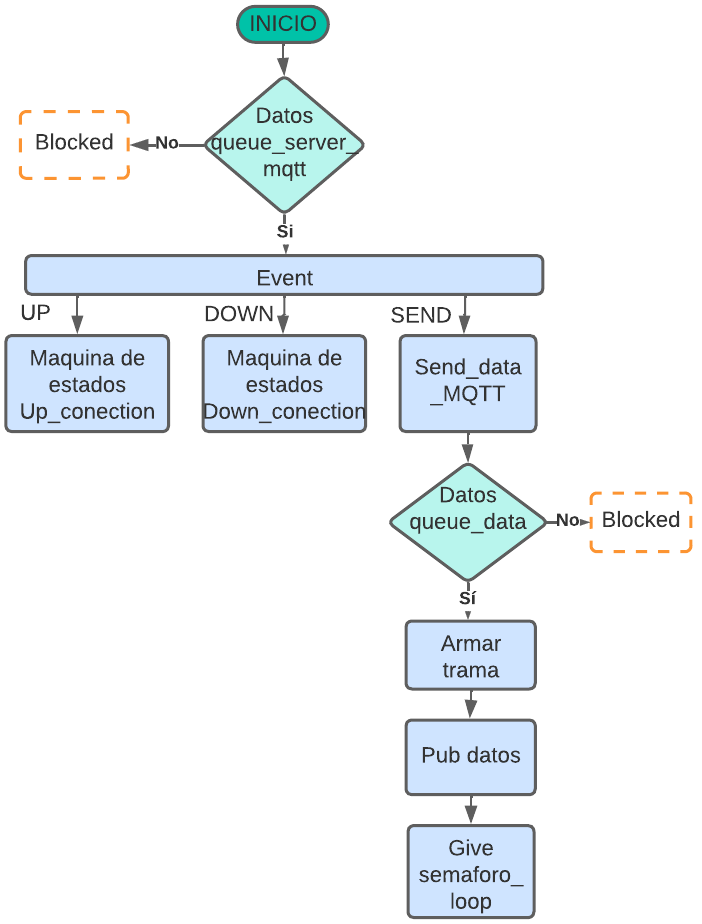
\includegraphics[width=8cm, height=8.5cm]{./Figures/DF general task conection.png}
	\caption{Diagrama de flujo tarea conexion server MQTT.}
	\label{fig:Df tarea conexion}
\end{figure}

\begin{figure}[h]
  \centering
  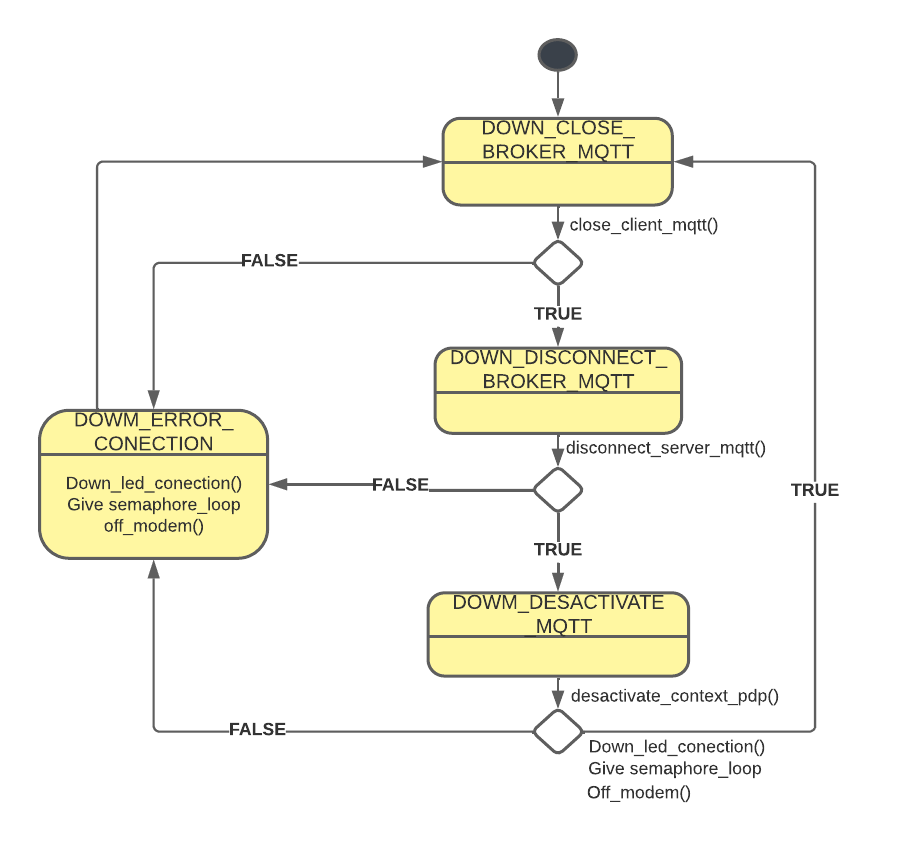
\includegraphics[width=8cm, height=8cm]{./Figures/SM down server.png}
  \caption{Maquina de estados down servidor.}
  \label{fig:Maquina de estados dowm servidor}
\end{figure}
\clearpage
\hspace{0.5cm}

\begin{figure}[t!]
  \centering
	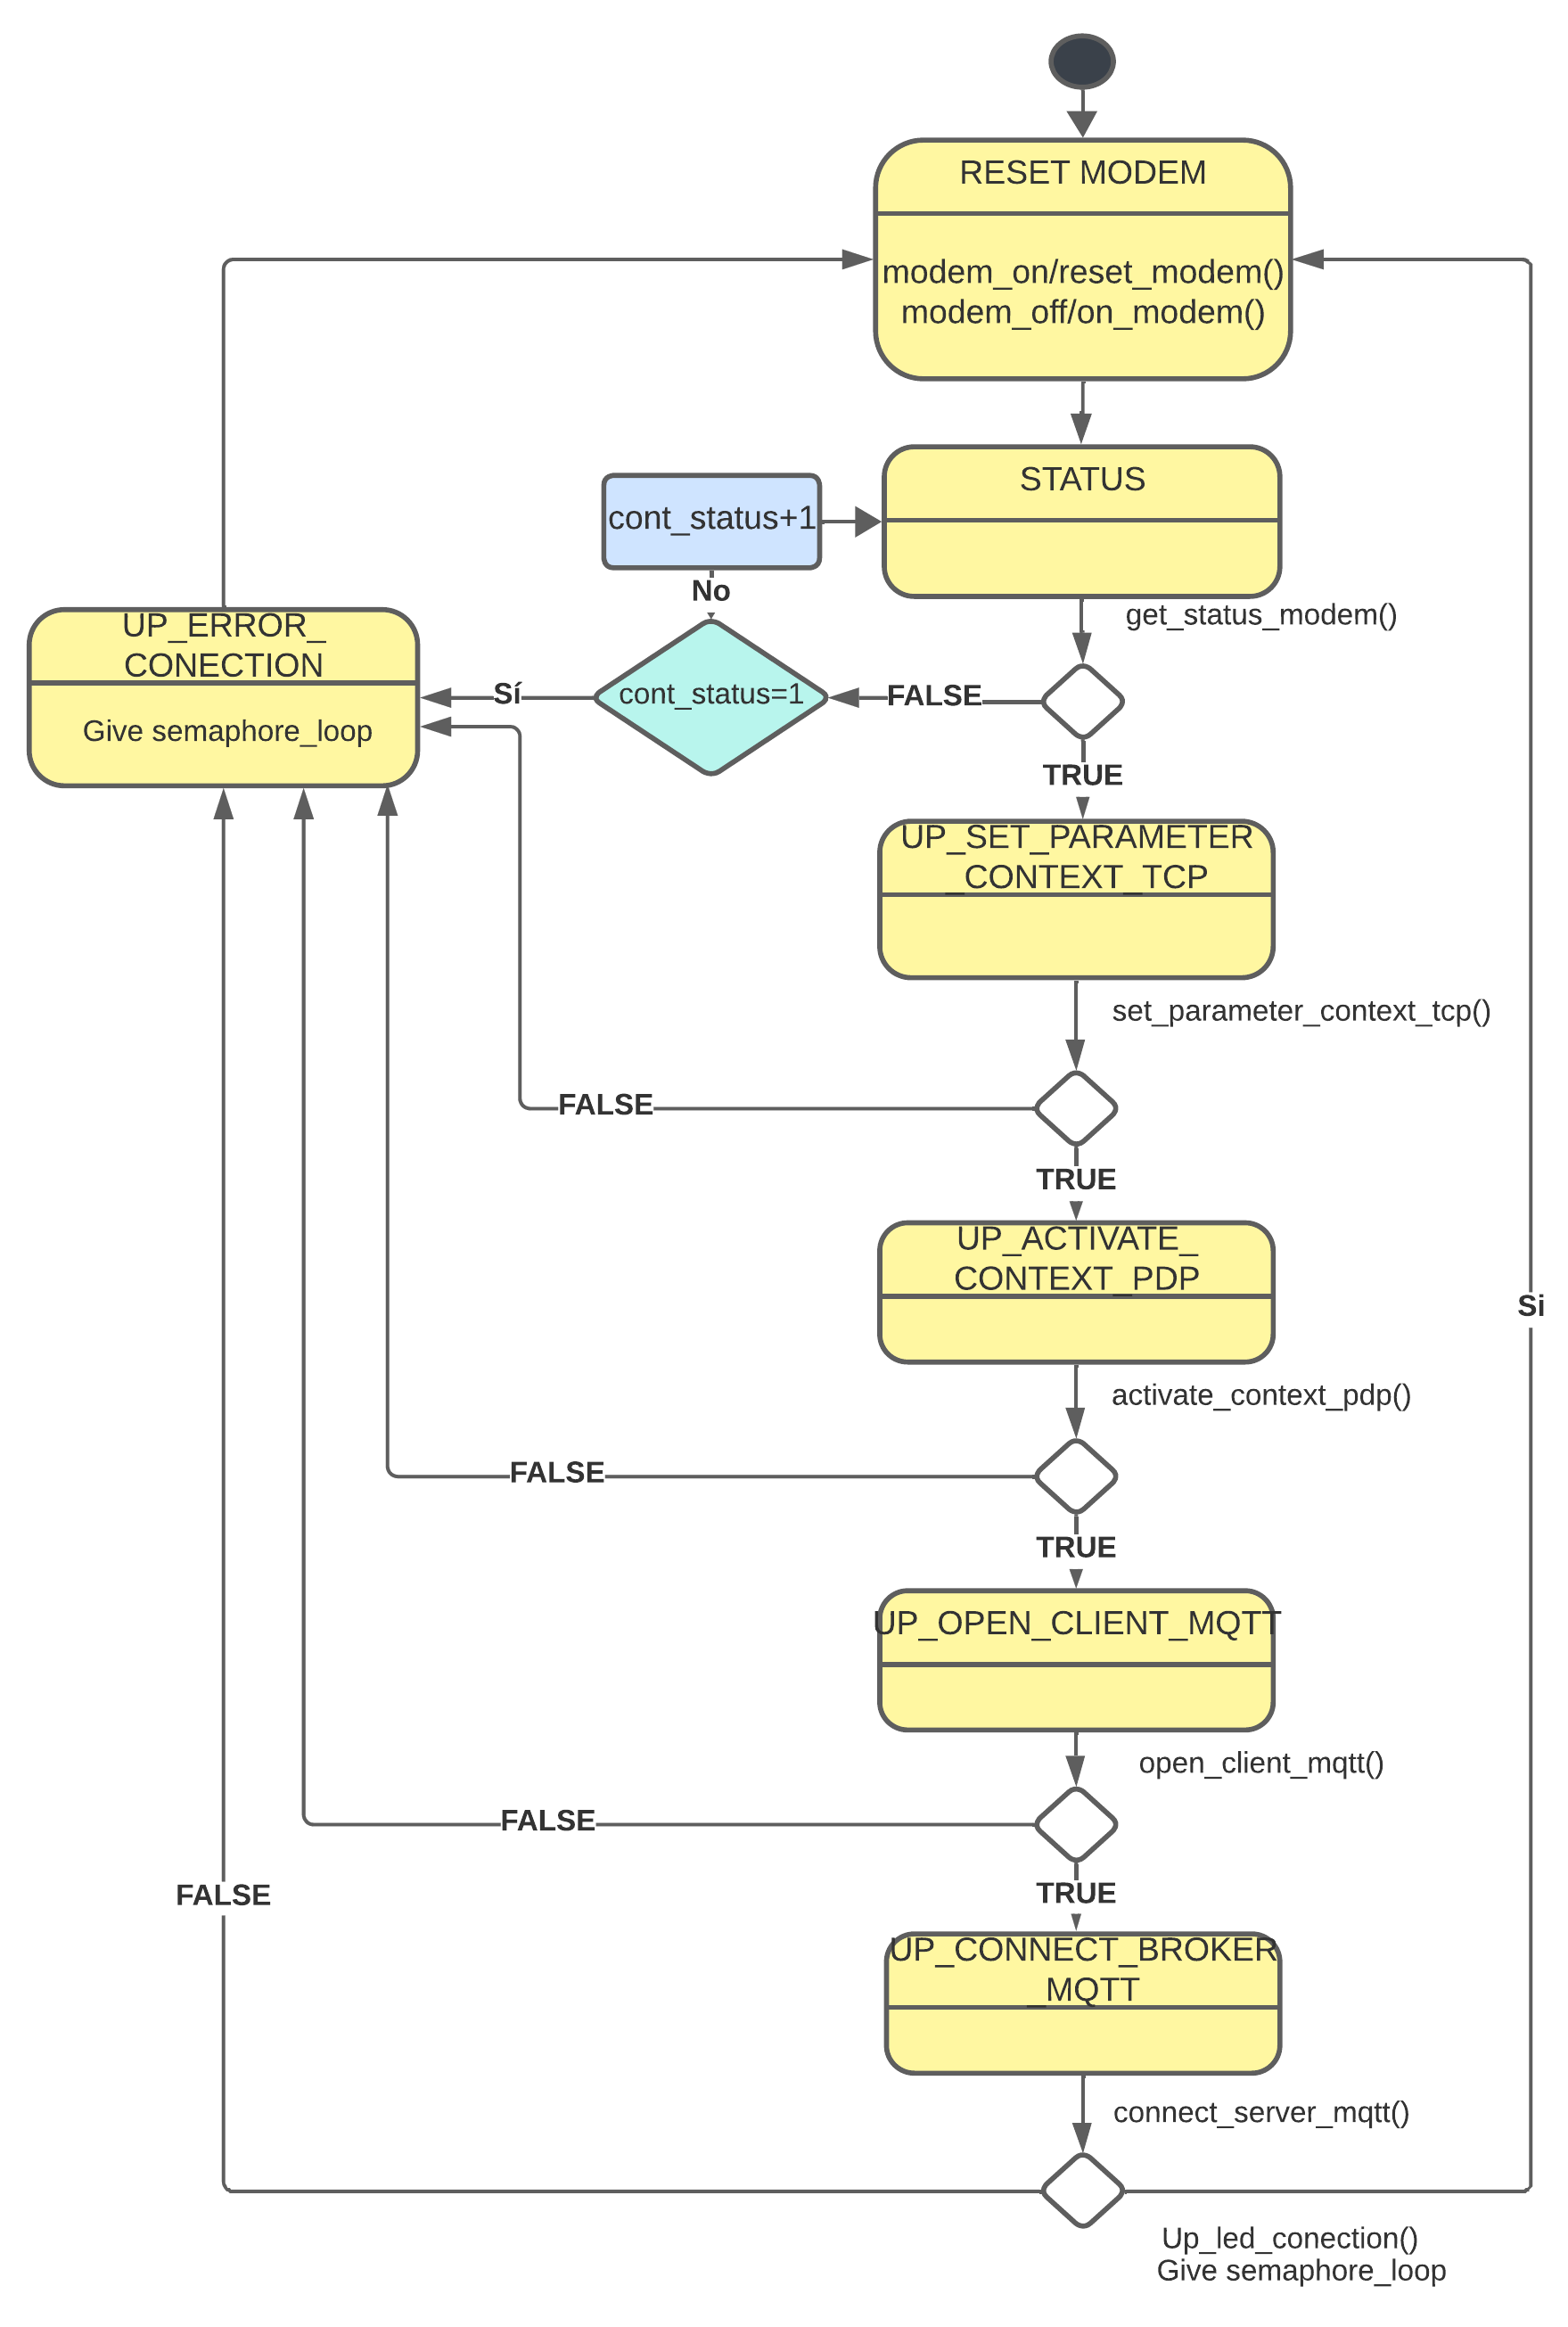
\includegraphics[width=10cm, height=14cm]{./Figures/SM up server.png}
	\caption{Maquina de estados up servidor.}
	\label{fig:Maquina de estados up servidor}
\end{figure}

\section{Controladores implementados}
Se implementaron dos controladores para el modulo de comunicacion BG96 y para el sensor de humedad y temperatura ambiente AHT-10.

\subsection{Controlador sensor AHT10} 
En el codigo \ref{cod:codigo AHT10} se ven las funciones mas utilizadas del driver en el firmware.

\begin{lstlisting}[label=cod:codigo AHT10,caption=Funciones principales del driver del sensor AHT10.]  % Start your code-block

//Estructura para manejar los datos del driver del sensor    
typedef struct 
{
  aht10WriteFcn_t  writeI2C;
  aht10ReadFcn_t  readI2C;
  delay1ms_t      delay_ms_I2C;    
  aht10_status_fnc status_fun;
}aht10_config_t;

//Funcion para inicializar el driver 
void aht10Init(aht10_config_t *obj, aht10WriteFcn_t fncWritePort, aht10ReadFcn_t fncReadPort, delay1ms_t fncDelayPort)
{
  obj->writeI2C=fncWritePort;
  obj->readI2C=fncReadPort;
  obj->delay_ms_I2C=fncDelayPort;
}
//Funcion para obtener el valor de la humedad leida por el sensor 
aht10_status_fnc aht10_get_humedity(aht10_config_t*obj, uint8_t *data)
{
  if (obj== NULL)
  {
    return AHT10_ERROR;
  }
  obj->status_fun=AHT10_ERROR;
  uint8_t bufferRead[6]={0};
  uint32_t data_humedity=0;
  obj->status_fun=aht10_launch_measurement(obj);
  if (obj->status_fun==AHT10_OK)
  {
    obj->status_fun= obj->readI2C(AHT10_ADDRESS_SLAVE,bufferRead,6);
    if (obj->status_fun==AHT10_OK)
    {
      data_humedity=(((uint32_t)bufferRead[1]<<16) | ((uint16_t)bufferRead[2]<<8) | (bufferRead[3]))>>4;
      *data= HUMEDITY(data_humedity);
    }
  }
  return obj->status_fun;
}
//Funcion para obtener el valor de la temperatura leida por el sensor 
aht10_status_fnc aht10_get_temperature(aht10_config_t*obj, int8_t *data)
{
  if (obj== NULL)
  {
    return AHT10_ERROR;
  } 
  uint8_t buffer_read[6]={0};
  uint32_t data_temperature=0;
  obj->status_fun=AHT10_ERROR;
  obj->status_fun=aht10_launch_measurement(obj);
  if (obj->status_fun==AHT10_OK)
  {
    obj->status_fun=obj->readI2C(AHT10_ADDRESS_SLAVE ,buffer_read,6);
    if (obj->status_fun==AHT10_OK)
    {
      data_temperature=((uint32_t)(buffer_read[3] & 0x0F)<<16) | ((uint16_t) buffer_read[4]<<8)| buffer_read[5];
      *data= TEMPERATURE(data_temperature);
    }
  }
  return obj->status_fun;
}
\end{lstlisting}
\subsection{Controlador modulo de comunicacion BG96 } 
En el codigo \ref{cod:driver bg96} se muestran las funciones mas utilizadas por el firmware del driver que son las de configuracion y activacion del APN, conexion y desconexion al servidor MQTT.

\begin{lstlisting}[label=cod:driver bg96,caption=Funciones principales del driver del sensor AHT10.]  % Start your code-block

//Estructura para manejar los datos del driver 
typedef struct 
{
  em_status_modem  status_modem;
  em_state_server_mqtt_conection status_mqtt_server;
  pf_send_data    send_data_device;
  pf_reset_modem  f_reset_modem; 
  st_config_parameters_mqtt self_mqtt;
  st_config_context_tcp self_tcp;
  st_info_product info_product;
  uint8_t           last_error;
  char buffer_resp [100];
  char *current_cmd;
  em_bg96_error_handling ft_resp;
}st_bg96_config;

//Funcion de inicio del driver 
em_bg96_error_handling init_driver(st_bg96_config *self,pf_send_data ft_send_data_device,pf_reset_modem ft_reset_modem)
{
  if (ft_send_data_device!=NULL) {
    self->send_data_device=ft_send_data_device;
  }
  if (ft_reset_modem!=NULL) {
    self->f_reset_modem=ft_reset_modem;
  }
    self->status_modem=OFF;
    self->ft_resp=FT_BG96_OK;
    self->last_error=BG96_NO_ERROR;
    self->self_tcp.context_id=1;
    self->self_tcp.context_type=1;
    self->self_tcp.method_authentication=1;
    self->self_tcp.tcp_password="";
    self->self_tcp.tcp_username="";
    self->self_mqtt.identifier_socket_mqtt=0;
    self->self_mqtt.quality_service=0;
    self->self_mqtt.port=1883;
    self->self_mqtt.mqtt_client_id="123a56cb9";
    self->status_mqtt_server=SERVER_MQTT_DOWN;
    self->self_mqtt.host_name="\"mqtt.thingsboard.cloud\"";
    self->self_mqtt.mqtt_username="";
    self->self_mqtt.mqtt_password="";
    self->self_tcp.tcp_apn="internet.tigo.bol";
    return self->ft_resp;
}
//Funcion para saber el estado del modulo
em_bg96_error_handling get_status_modem(st_bg96_config* self)
{
  self->ft_resp=FT_BG96_OK;
  self->current_cmd="AT\r";
  self->ft_resp=self->send_data_device(self->current_cmd,RS_BG96_OK,self->buffer_resp,1000);
  if (self->ft_resp!=FT_BG96_OK)
  {
    self->last_error=BG96_ERROR_STATUS_MODEM;
  }
  return self->ft_resp;
}
//Funcion para enviar mensaje de texto 
em_bg96_error_handling send_sms_bg96(st_bg96_config *self,char*number,char*message)
{
  self->ft_resp=FT_BG96_OK;
  char buffer_message[256];
  char buffer_number[20];
  sprintf(buffer_number,"AT+CMGS=\"%s\"\r",number);
  sprintf(buffer_message,"%s\x1a\r",message);
  
  self->ft_resp=self->send_data_device(buffer_number,RS_BG96_SIGNAL,self->buffer_resp,12000);
  if (FT_BG96_OK==self->ft_resp)
  {
    self->ft_resp=self->send_data_device(buffer_message,RS_BG96_OK,self->buffer_resp,12000);
    if (FT_BG96_OK!=self->ft_resp)
    {
      self->last_error=BG96_ERROR_SEND_SMS;
    }
  }
  return self->ft_resp;
}
//Funcion para configurar el contexto de la red
em_bg96_error_handling set_parameter_context_tcp(st_bg96_config *self)
{   
  self->ft_resp=FT_BG96_OK;
  char cmd[100];
  sprintf(cmd,"AT+QICSGP=%u,%u,\"%s\",\"%s\",\"%s\",%u\r",self->self_tcp.context_id,self->self_tcp.context_type,self->self_tcp.tcp_apn,self->self_tcp.tcp_username,self->self_tcp.tcp_password,self->self_tcp.method_authentication);
  self->ft_resp=self->send_data_device(cmd,RS_BG96_OK,self->buffer_resp,3000);
  if (self->ft_resp!=FT_BG96_OK)
  {
    self->last_error=BG96_ERROR_SET_PARAMETER_CONTEXT_TCP;
  }
  return self->ft_resp;
}
//Funcion para activar el contexto pdp
em_bg96_error_handling activate_context_pdp(st_bg96_config *self)
{
  self->ft_resp=FT_BG96_OK;
  char cmd[30];
  sprintf(cmd,"AT+QIACT=%u\r",self->self_tcp.context_id);
  self->ft_resp=self->send_data_device(cmd,RS_BG96_OK,self->buffer_resp,15000);
  if (self->ft_resp!=FT_BG96_OK)
  {
    self->last_error=BG96_ERROR_ACTIVATE_CONTEXT_PDP;
  }
  return self->ft_resp;
}
//Funcion para abrir un cliente MQTT
em_bg96_error_handling open_client_mqtt(st_bg96_config *self)
{
  self->ft_resp=FT_BG96_ERROR;
  char cmd[100];
  sprintf(cmd,"AT+QMTOPEN=%u,%s,%u\r",self->self_mqtt.identifier_socket_mqtt,self->self_mqtt.host_name,self->self_mqtt.port);
  self->ft_resp=self->send_data_device(cmd,RS_BG96_CERO,self->buffer_resp,75000);
  if (self->ft_resp!=FT_BG96_OK)
  {
    self->last_error=BG96_ERROR_OPEN_CLIENT_MQTT;
  } 
  return self->ft_resp;
}
//Funcion para conectarse al servidor MQTT
em_bg96_error_handling connect_server_mqtt(st_bg96_config *self)
{
  self->ft_resp=FT_BG96_ERROR;
  char cmd[150]={0};
  sprintf(cmd,"AT+QMTCONN=%u,\"%s\",\"%s\",\"%s\"\r",self->self_mqtt.identifier_socket_mqtt,self->self_mqtt.mqtt_client_id,self->self_mqtt.mqtt_username,self->self_mqtt.mqtt_password);
  self->ft_resp=self->send_data_device(cmd,RS_BG96_CERO,self->buffer_resp,10000);
  if (self->ft_resp!=FT_BG96_OK)
  {
    self->last_error=BG96_ERROR_CONNECT_SERVER_MQTT;
  }
  return self->ft_resp;
}
//Funcion para publicar un mensaje al topico configurado 
em_bg96_error_handling publish_message(st_bg96_config *self,char *topic,char *data)
{
  self->ft_resp=FT_BG96_ERROR;
  char cmd[50]={0};
  char buffer_data[220]={0};
  sprintf(buffer_data,"%s\x1a\r",data);
  sprintf(cmd,"AT+QMTPUB=%u,0,0,0,\"%s\"\r",self->self_mqtt.identifier_socket_mqtt,topic);
  self->ft_resp=self->send_data_device(cmd,RS_BG96_SIGNAL,self->buffer_resp,3000);
  if (FT_BG96_OK==self->ft_resp)
  {
    self->ft_resp=self->send_data_device(buffer_data,RS_BG96_CERO,self->buffer_resp,15000);
    if (self->ft_resp!=FT_BG96_OK)
    {
      self->last_error=BG96_ERROR_PUBLISH_MESSAGE;
    }   
 }
    else self->last_error=BG96_ERROR_PUBLISH_MESSAGE;
    return self->ft_resp;
}


\end{lstlisting}
\clearpage
\section{Desarrollo del hardware}

Para diseño del hardware se utilizo KICAD 6.0 herramienta de diseño aprendida en transcurso de  la especialización.

\subsection{Esquematico} 
Al ser un prototipo lo que se hizo fue desarrollar un tarjeta donde se puedan ensamblar y conectar nuestros módulos utilizados en el proyecto: módulo de comunicación celular, tarjeta de desarrollo con el microcontrolador y  los módulos sensores.

En la figura \ref{fig:esquematico root} se muestra la página raíz del esquemático del proyecto, en la parte izquierda superior se  ven la número de hojas en las que se dividió el esquemático, en la parte izquierda inferior se ve el 3d del la tarjeta desarrollada y en parte derecha se ve la conexión entre las diferentes hojas del proyecto.

\begin{figure}[h]
  \centering
	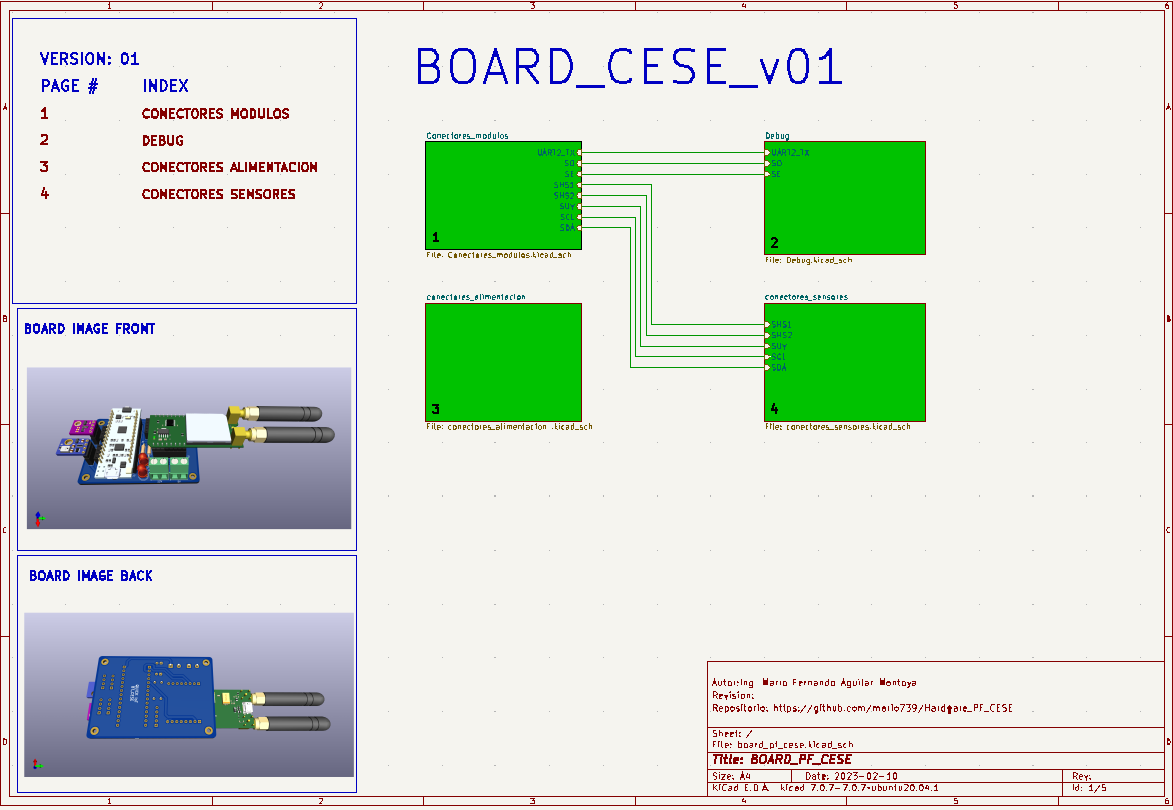
\includegraphics[width=\textwidth, height=8cm]{./Figures/esquematico_root.png}
	\caption{Esquematico pagina raiz.}
	\label{fig:esquematico root}
\end{figure}

En figura \ref{fig:esquematico modulos} se muestra los conectores de los módulos más importantes: el módulo de comunicación BG96, módulo NUCLEO-L432KC y la conexión entre ellos.

\begin{figure}[h]
  \centering
	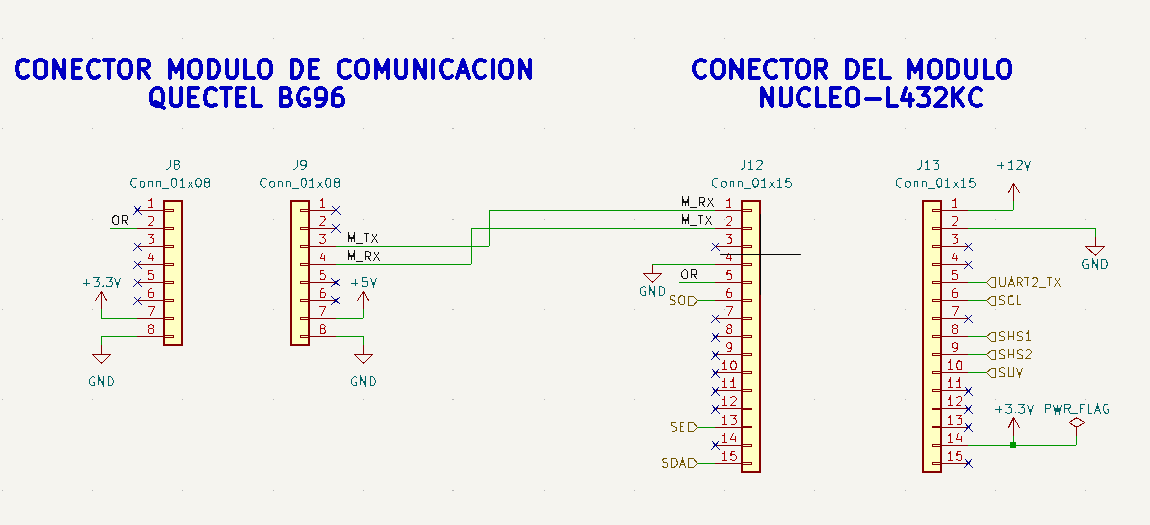
\includegraphics[width=10cm, height=5cm]{./Figures/esquematico_modulos.png}
	\caption{Esquematico conectores modulos.}
	\label{fig:esquematico modulos}
\end{figure}

Se colocaron dos leds para debug, uno para señalizar si se logró conectar al servidor MQTT y el otro led para señalizar si el sistema entra en un estado de error, se colocó un conector para una puerto serial por donde el módulo manda la secuencias de comandos que manda y recibe del módulo de comunicación. En la figura \ref{fig:esquematico conectores de debug} se puede ver el circuito.
\begin{figure}[h!]
  \centering
	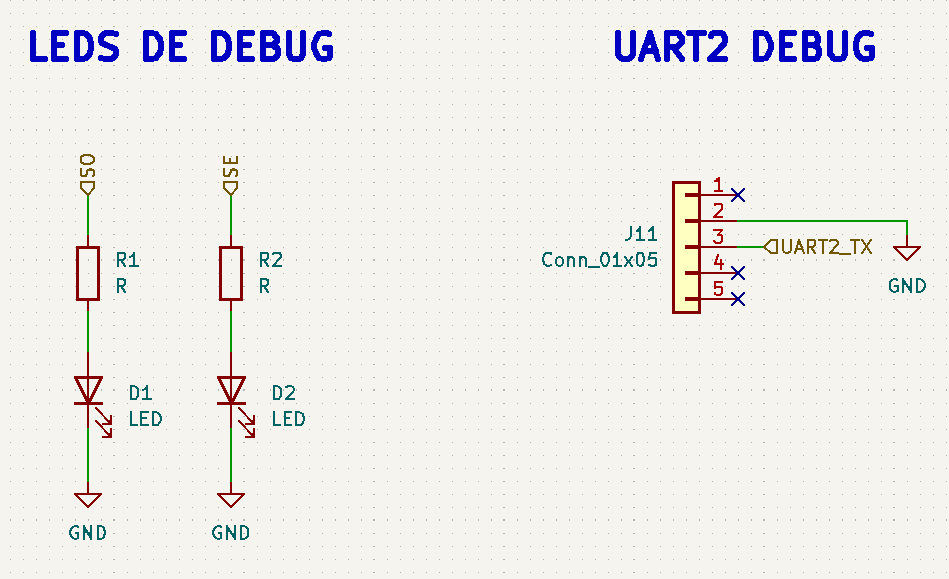
\includegraphics[width=10cm, height=4cm]{./Figures/esquematico_debug.png}
	\caption{Esquematico interfaz de debug.}
	\label{fig:esquematico conectores de debug}
\end{figure}

En la figura \ref{fig:esquematico conectores sensores} se pueden ver los conectores que se colocaron a la placa para conectar los sensores del nodo: sensor de humedad 1, sensor de humedad 2, sensor de luz UV y el sensor de humedad y temperatura ambiente AHT-10.
\begin{figure}[h]
  \centering
	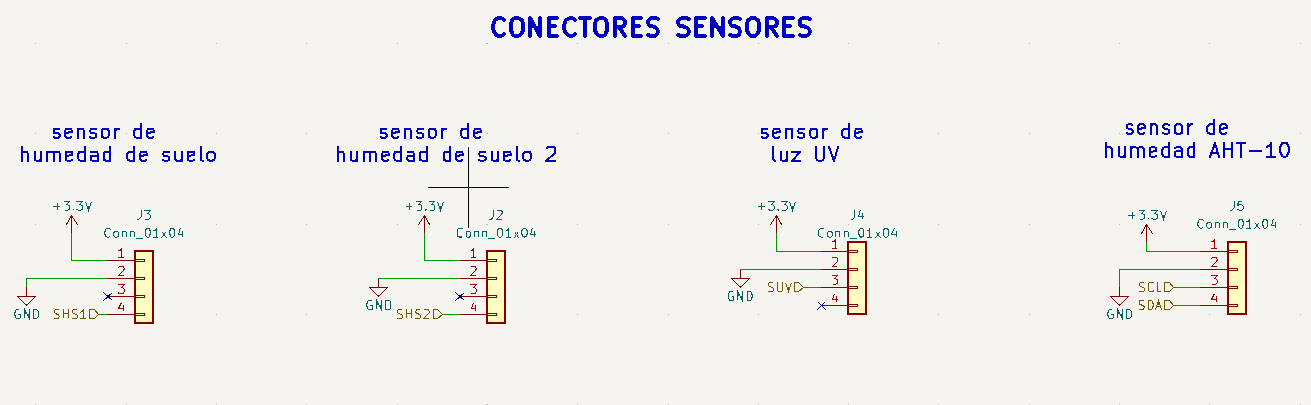
\includegraphics[width=10cm, height=4.5cm]{./Figures/esquematico_conectores_sensores.png}
	\caption{Esquematico conectores sensores.}
	\label{fig:esquematico conectores sensores}
\end{figure}

Se colocaron dos colectores de alimentación como se muestra en la figura \ref{fig:esquematico conectores alimentacion}, el conector de 12v para alimentar al módulo del microcontrolador y el otro conector para alimentar al módulo de comunicación.
\begin{figure}[h]
  \centering
	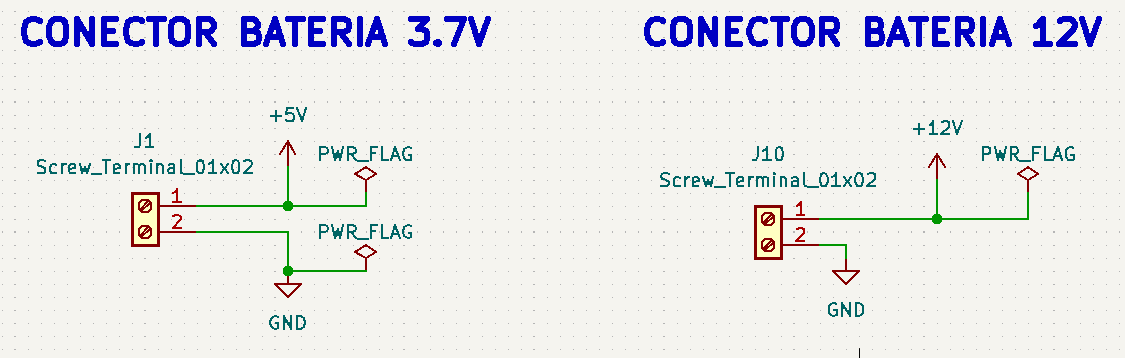
\includegraphics[width=10cm, height=4.5cm]{./Figures/esquematico_alimentacion.png}
	\caption{Esquematico conectores alimentacion.}
	\label{fig:esquematico conectores alimentacion}
\end{figure}

\subsection{PCB del hardware} 
La figura \ref{fig:PCB del proyecto} muestra el circuito impreso diseñado para el proyecto.

\begin{figure}[h!]
  \centering
  \begin{subfigure}[b]{0.28\linewidth}
  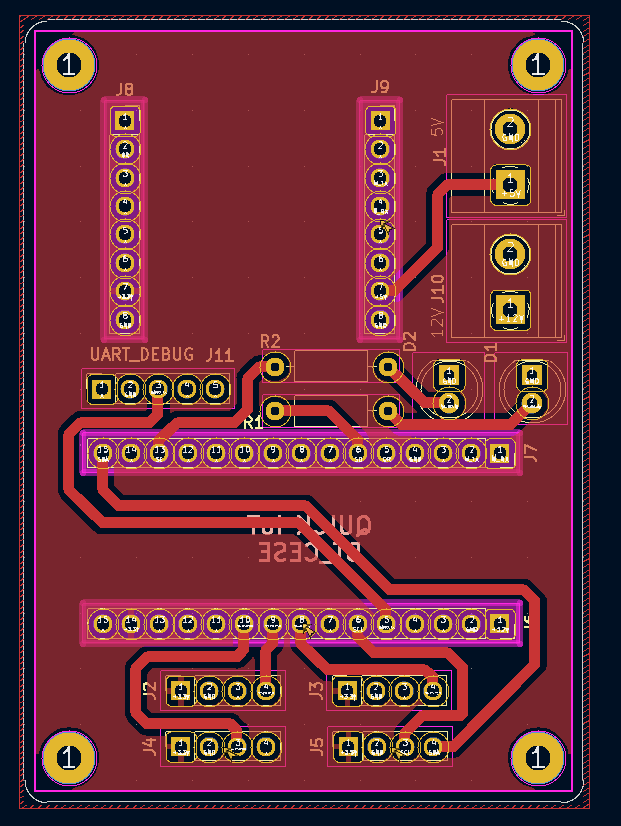
\includegraphics[width=\linewidth]{./Figures/pcb_top.png}
  \caption{Capa top PCB}
  \label{fig:Capa top PCB}
  \end{subfigure}
  \begin{subfigure}[b]{0.27\linewidth}
  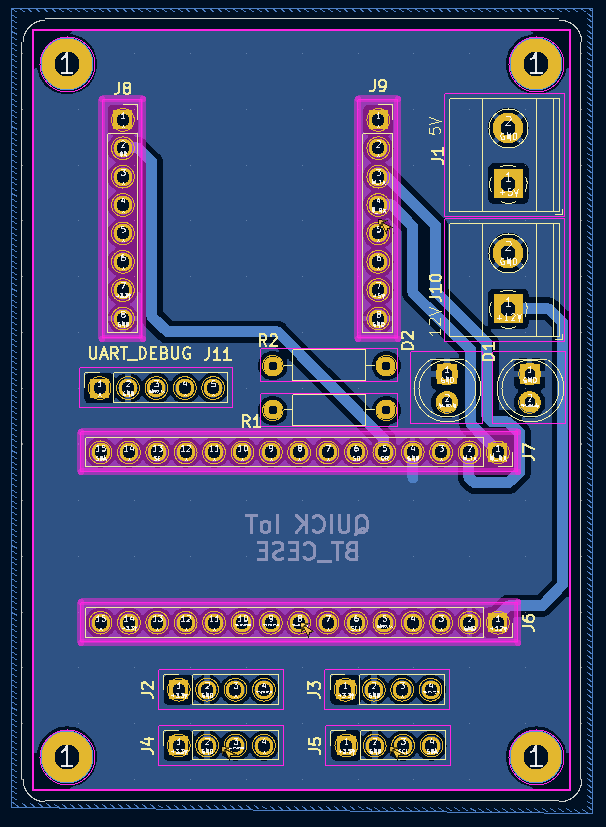
\includegraphics[width=\linewidth]{./Figures/pcb_bot.png}
  \caption{Capa bot PCB}
  \label{fig:Capa bot PCB}
  \end{subfigure}
  \caption{PCB del proyecto.}
  \label{fig:PCB del proyecto}
  \end{figure}

En la figura \ref{fig:3D del modulo} se muestra del diseño de la tarjeta del circuito impreso en 3D.
\begin{figure}[h!]
  \centering
	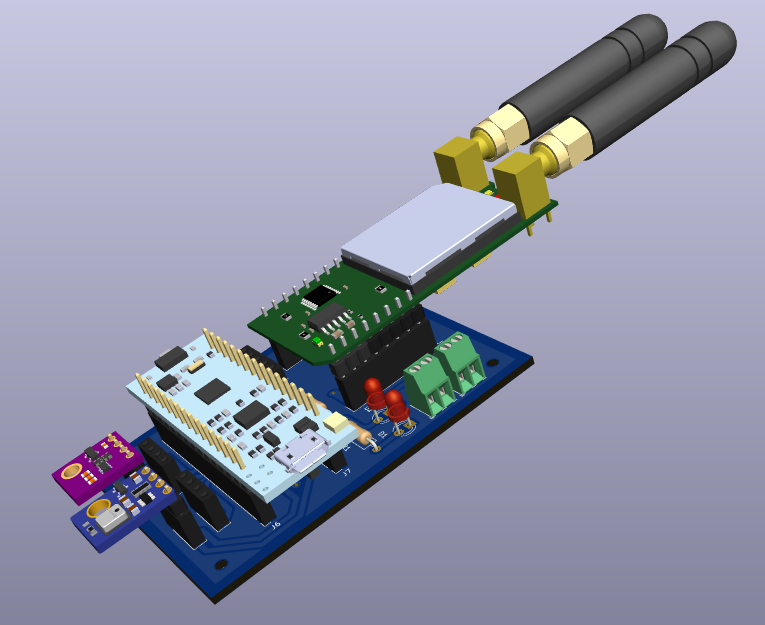
\includegraphics[width=8cm, height=4.5cm]{./Figures/tarjeta3d.png}
  \caption{3D del tarjeta desarrollada.}
	\label{fig:3D del modulo}
\end{figure}
\subsection{Fabricacion circuito impreso} 
Una vez completado y validado el diseño, se generaron los archivos de fabricación para su posterior producción por la empresa JLCPCB figura \ref{fig:PCB ensamblado}. 
\begin{figure}[h!]
  \centering
	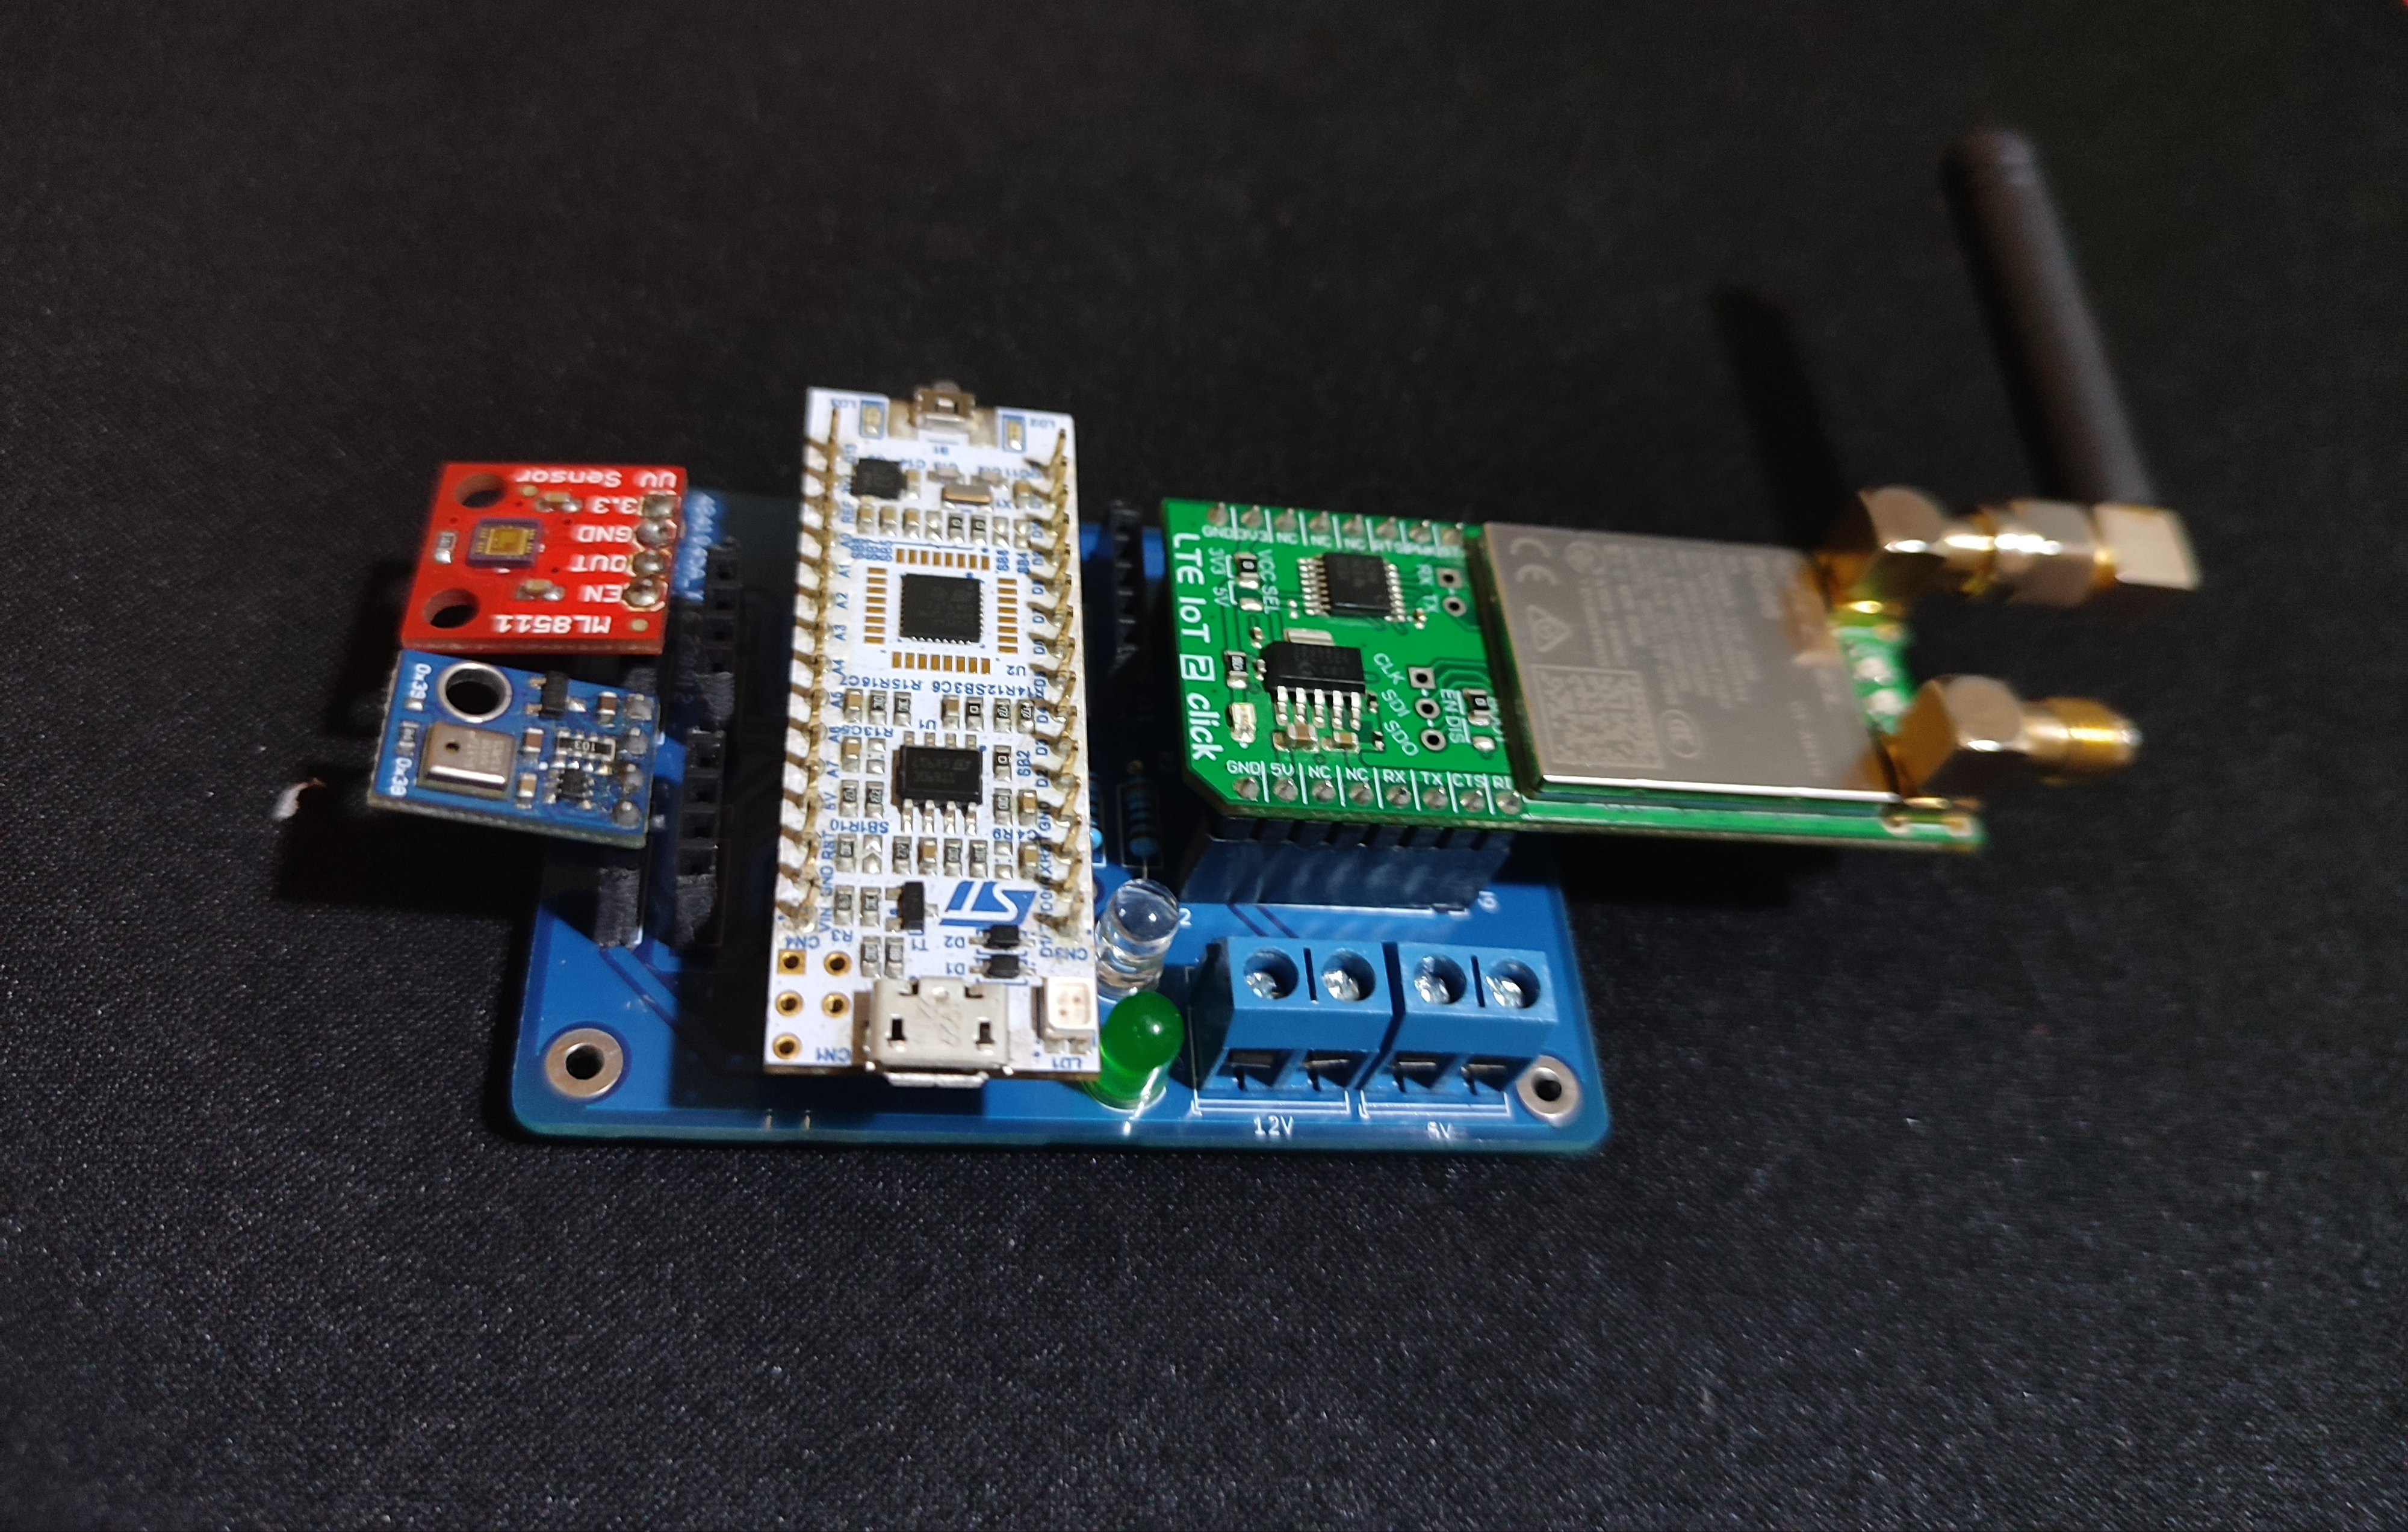
\includegraphics[width=8cm, height=5.5cm]{./Figures/hardware_vistalateral.jpg}
  \caption{PCB ensamblado.}
	\label{fig:PCB ensamblado}
\end{figure}

\clearpage
\section{Paneles de visualizacion}
La herramienta de visualización de ThingsBoard es muy versátil para el armado de paneles de visualización escalables y altamente configurables.

Se armaron dos paneles de visualización un panel principal que muestra todos los nodos sensores implementados y un panel secundario o panel de nodo sensor que muestra de forma detallada las variables monitoreadas por el nodo sensor.

\subsection{Panel principal} 

En la figura \ref{fig:Panel principal} se aprecia el panel principal de la interfaz gráfica.A continuación se describirán cada zona del panel principal.
El panel está dividido en las siguientes zonas:
\begin{itemize}
  \item Zona 1: Listado de todos los nodos sensores implementados y activos, asiendo click en el dispositivo podemos navegar al panel de visualización del nodo donde podemos ver con mas detalle las variables medidas.
  \item Zona 2: Gráficas que muestra los cambios que van teniendo los valores de las variables medidas por los sensores con respecto al tiempo.
  \item Zona 3: Mapa con la ubicación de los nodo sensores implementados.
\end{itemize}

\begin{figure}[h]
  \centering
	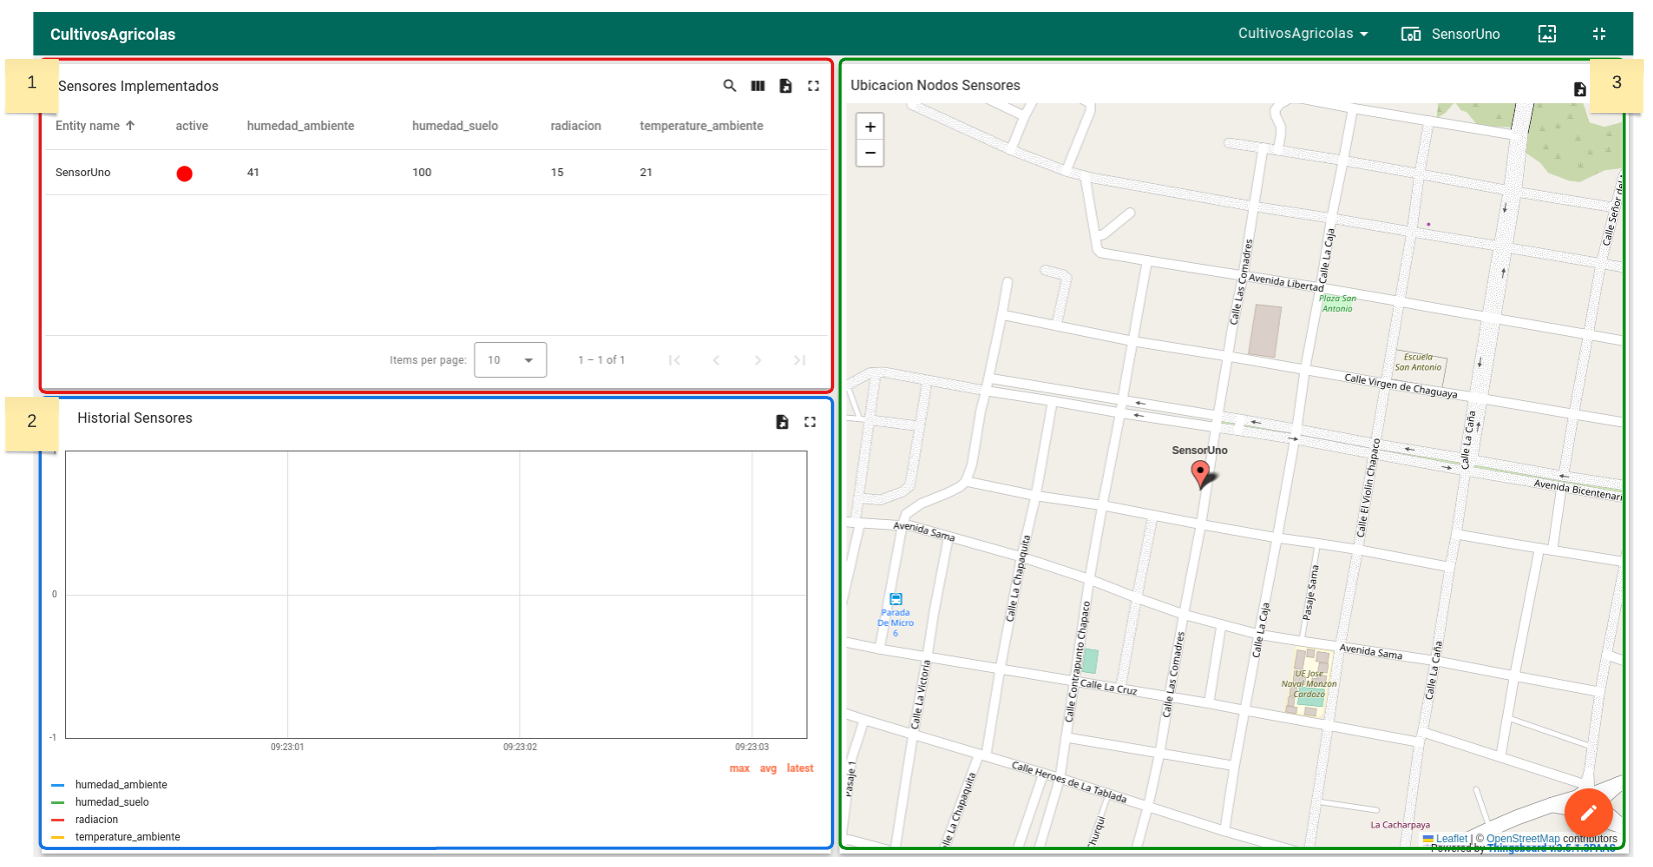
\includegraphics[width=\textwidth, height=11cm]{./Figures/panel_principal_editado.png}
  \caption{Panel principal de la interfaz grafica.}
	\label{fig:Panel principal}
\end{figure}

\clearpage
\subsection{Panel nodo sensor} 

Para tener un mayor detalle de todos los parámetros de monitoreo de cada nodo sensor se creo un panel secundario que se muestra en la figura \ref{fig:Panel nodo sensor}.

El panel esta dividido en las siguientes zonas:
\begin{itemize}
  \item Zona 1: Graficas que muestra los cambios que van teniendo los valores de las variables medidas por los sensores con respecto al tiempo.
  \item Zona 2: Widgets que muestran el último valor obtenido por el nodo sensor de cada variable monitoreada.
  \item Zona 3: Tabla que monitorea las alarmas implementadas. 
  \item Zona 4: Se tiene un mapa que muestra la ubicación del nodo sensor.
\end{itemize}

\begin{figure}[h!]
  \centering
	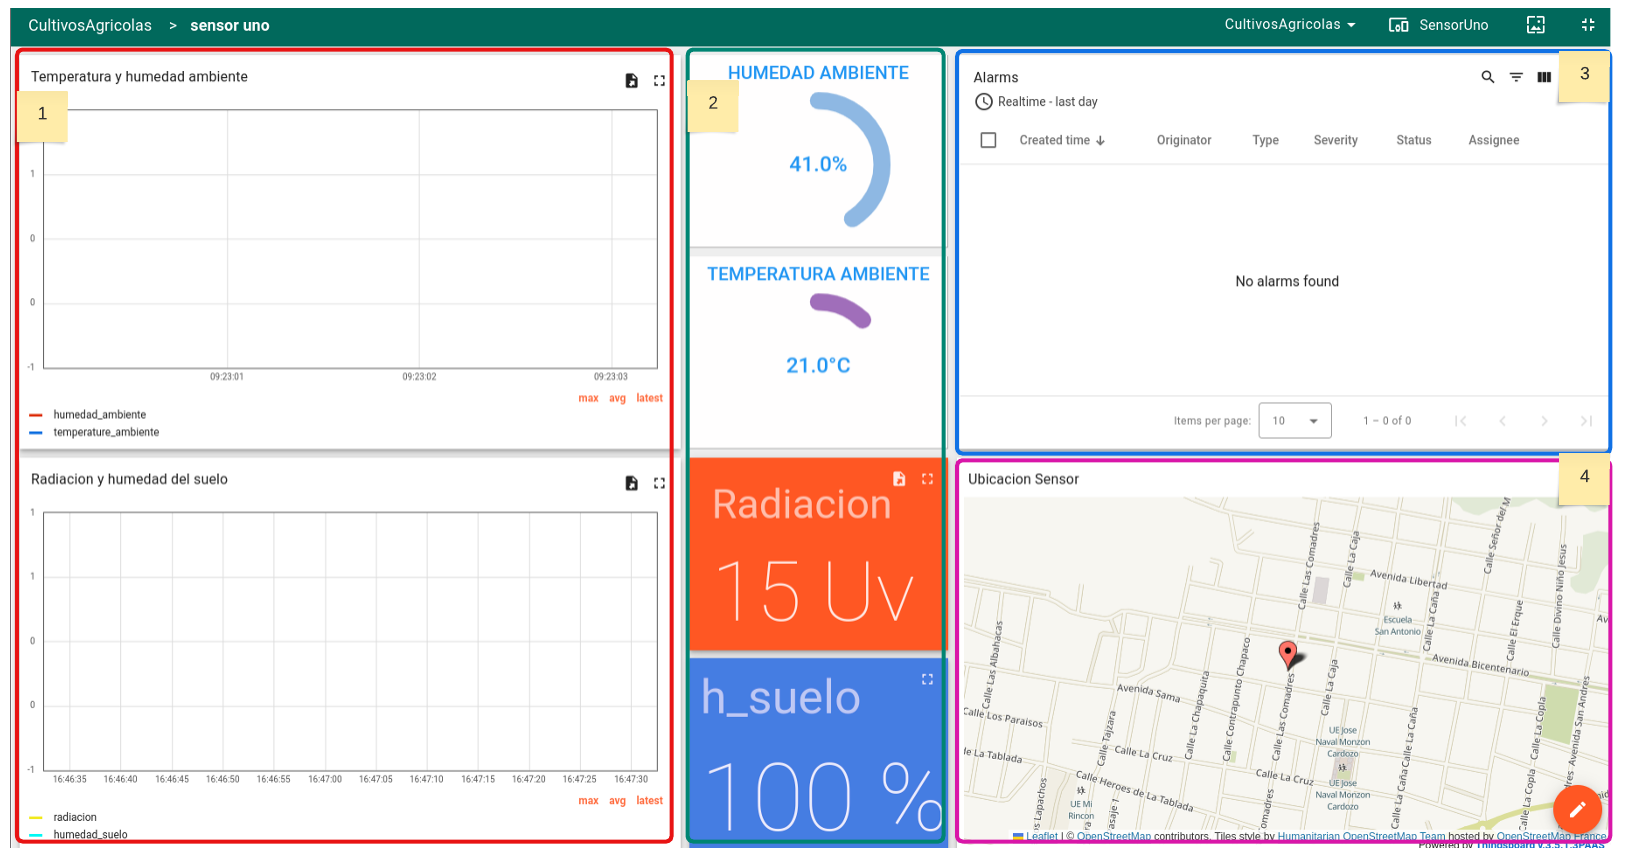
\includegraphics[width=\textwidth, height=10cm]{./Figures/panel_nodosensor_editado.png}
  \caption{Panel nodo sensor.}
	\label{fig:Panel nodo sensor}
\end{figure}